\documentclass[12pt]{report}

\usepackage[utf8]{inputenc}
\usepackage{graphicx}
\graphicspath{ {images/} }
\usepackage{float}

\usepackage[a4paper,width=150mm,top=25mm,bottom=25mm]{geometry}

\usepackage{fancyhdr}
\pagestyle{fancy}

% For citations
\usepackage[backend=bibtex]{biblatex}
\addbibresource{Final_Paper.bib}
\usepackage{hyperref}
\hypersetup{
  linkcolor=blue,
  citecolor=blue
}
\hypersetup{colorlinks=true,linkcolor=blue}
% For citations and urls in captions
\usepackage{caption}


\title{
  {Ethernet on the Zynq ZC706 \vspace{0.2in}}\\
  {\large 18-545 Advanced Digital Design \vspace{0.2in}}\\
  {
\includegraphics[width=2in]{cmu_seal.png}}
}

\author{Terence An, Eddie Nolan, Dale Zhang}
\date{December 12, 2015}

\begin{document}
\maketitle

\chapter{Introduction}
This paper is a guide to start building ethernet on the Zynq ZC706 board. It was originally written as the final project for a 18-545 project which didn't complete because they struggled to build an ethernet adapter in programmable logic and have it properly communicate with the Processing System. The intention of this paper is to aid future groups in completing an ethernet adapter, as well as providing the necessary background and deterring groups from fruitless avenues. This guide will expect a very minimal understanding of Vivado because most students in 18-545 have had very limited exposure to Vivado. We will attempt to provide the pertinent references as needed.

That being said, going through Lab 2 in \textit{Vivado Design Suite Tutorial} \cite{vivado_tut} will probably be the fastest way to understand the work flow. Also, chapter 2 and chapter 4 of \textit{UltraFast Design Methodology Guide for the Vivado Design Suite} \cite{ultrafast} will be superbly helpful in learning to use Vivado, especially for using Intellectual Property (IP) in Vivado. Finally, if you still want more details on using IP, you can refer to the Vivado guide on \textit{Designing with IP} \cite{IP} and \textit{Designing IP Subsystems Using IP Integrator} \cite{IP_subsystems}. If you'd like more information on Vivado in general, refer to the \textit{Getting Started} \cite{starter} guide and the \textit{Designs Flows Overview} \cite{design_flows}.

\chapter{Ethernet Background}
In this chapter we'll provide the basics of ethernet, just enough to get you started.
Our discussion will start at the lowest level, and work our way up to the peripheral port on the processing system. If any of these sections are found to be lacking, you can find more information from the 802.3ab standard available on the \href{http://standards.ieee.org/about/get/802/802.3.html}{IEEE Standard Association}. Wikipedia is also your friend.
While the intention of this book is to help you build your own ethernet,
we dissuade people from actually implementing the physical transmission circuitry (PHY) yourself (the PCS and the PMA). The PMA layer is reasonable, but the PCS layer is incredibly involved. If that is all you intend to build for the semester, then perhaps it is possible. Instead we recommend you use the Vivado IP. So we'll simply provide an overview of what these parts do, and if you'd like to build these subsystems yourself, you'll have to refer to the 802.3 documentation.

\section{Logical Link Layer}
The logical link layer may also be referred to as the physical layer.
This network layer deals with how the bits are formatted into frames and how they're transmitted.
If you've worked on any networking projects previously, you could probably just skip this section.

\subsection{Ethernet Frame}
In Figure \ref{fig:eframe} you can see the basic format. However, there is another format for supporting larger frames called jumbo frames, so if frames don't look like what you're expecting that is a possibility. But it isn't very likely, because although most switches and routers support jumbo frames, they're not widely used. While we show the format of the frame, the logical link layer doesn't ascribe any meaning to these bits.

\begin{figure}[!h]
\centering
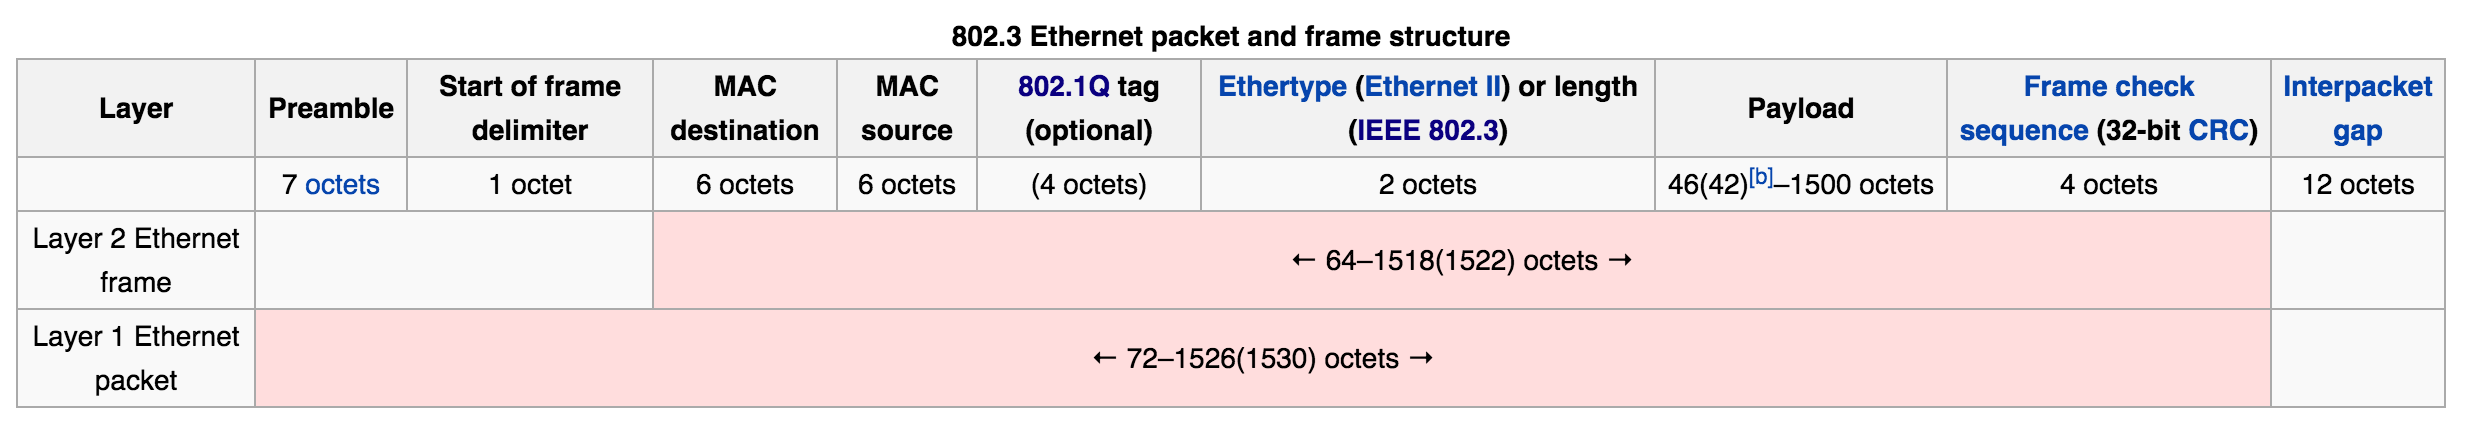
\includegraphics[width=6in]{eframe}
\caption{Ethernet Frame Format}
\small source:\url{https://en.wikipedia.org/wiki/Ethernet_frame}
\label{fig:eframe}
\end{figure}

The layer one bit sequence is what you'd expect to find on the wire, and the layer two format is what you'd expect to reach the operating system.

If there are other headers you're expecting, they'd be in the beginning of the payload. All information used by higher network layers would be found there as well. The standard maximum transmission unit is 1500 bytes, so if you're making a large download, it' be broken up into roughly 1500 byte chunks, each sent according to some highler level protocol like TCP or UDP and your application will receive them in these chunks.

Ethernet frames are sent across Cat-5 or Cat-6 cables, and you'll often see the cables referred to as full-duplex or half-duplex. Duplex refers to the two directions of traffic, tranmissions and receptions. A half-duplex cable/port alternates between transmit mode and receive mode, whereas a full-duplex cable/port has two seperate physical mediums allowing it to transmit and receive at the same time thus removing the need for any collision detection. You'll most likely be using the 1000Base-T standard (802.3ab, the twisted-pair copper standard for 1000Mbs as opposed to 1000Base-X, the fiber optic standard for 1000Mbs) which only operates on full-duplex.

The frame is transmitted 8 bits at a time over these wires, but they're encoded,
so if you wanted to parse these bits yourself it's a little bit more complicated.
We'll discuss more about this in the PMA section.

\subsection{Physical Medium Attachment (PMA)}
The PMA is the first subsystem that connects to the actual wires which is called the Medium Dependent Interface (MDI). The signals then are transmitted to a PCS PMA interface.
The PMA is fairly straight forward to implement, you simply have to properly implement a very brief transmit function, receive function, reset function, link monitor function, clock recovery function, and a fairly lengthly control function. The exact details can be found in the 802.3z standard, section 40.4.3. Figure \ref{fig:pma} gives a succinct overview of how the signals are used and generated.


The MDI consists of 4 wires for each transmission direction and each wire can take of 5
different voltages which we'll label as \{2,1,0,-1,-2\}.
The transmit side constantly changes the voltage, even when idle.
During idle, the voltages oscillate from 2 to 0 to -2 and back.
The baud rate is 125 MBaud which matches the clock rate of 125 MHz so there's one symbol per 8 ns.

\begin{figure}[H]
\centering
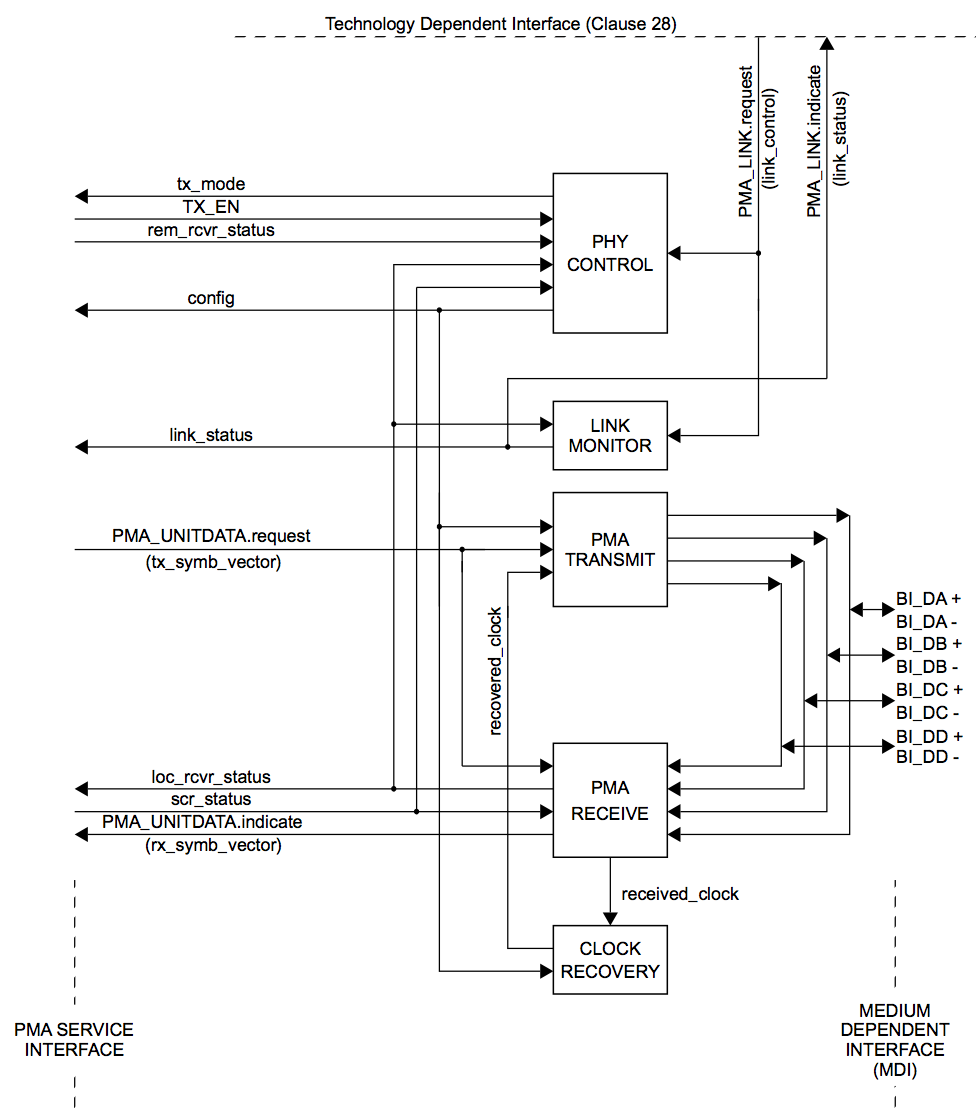
\includegraphics[width=4in]{pma}
\caption{PMA Reference Diagram}
\small source:802.3z Standard 40.4.3, Figure 40-13 \cite{802.3z}
\label{fig:pma}
\end{figure}

\subsection{Physical Coding Sublayer (PCS)}
The PCS is the subsystem that connects from the PMA to the Media Independent Interface (MII).
Because this guide is for 1000Base-T, our PCS must interface to Gigabit Media Independent Interface (GMII) or the Reduced GMII (RGMII).
In figure \ref{fig:pcs} you can see an overview of the PCS function. However, it hides a lot
of complexity. Implementing your own PCS is a very large undertaking,
despite the small reference diagram. It might appear as if you only have to implement
the transmit function, the transmit enable, collision detection, and the receive function.
The transmit function alone, is monumental.
We have to convert the bit stream into 4 wire code groups,
where each byte is encoded using the 4D-PAM5 technique into 4 quinary symbols.
We also have to scramble these symbols with a linear feedback shift technique.
The exact specifications can be found in section 40.3.1.3 in the 802.3z standard.
The state diagram can be seen in figure \ref{fig:pcs_transmit}.

\begin{figure}[H]
\centering
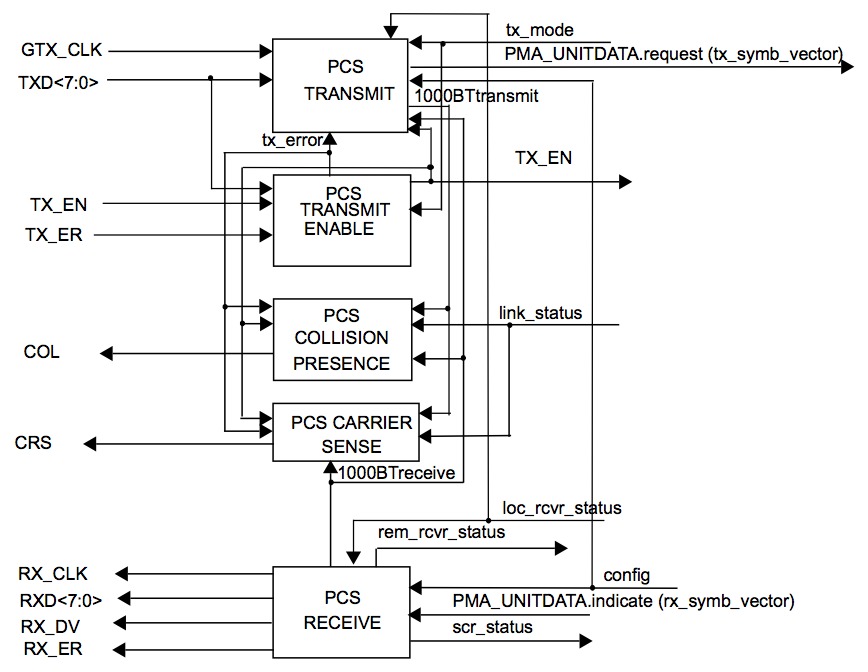
\includegraphics[width=4in]{pcs}
\caption{PCS Reference Diagram}
\small source:802.3z Standard 40.3.1, Figure 40-5 \cite{802.3z}
\label{fig:pcs}
\end{figure}

\begin{figure}[H]
\centering
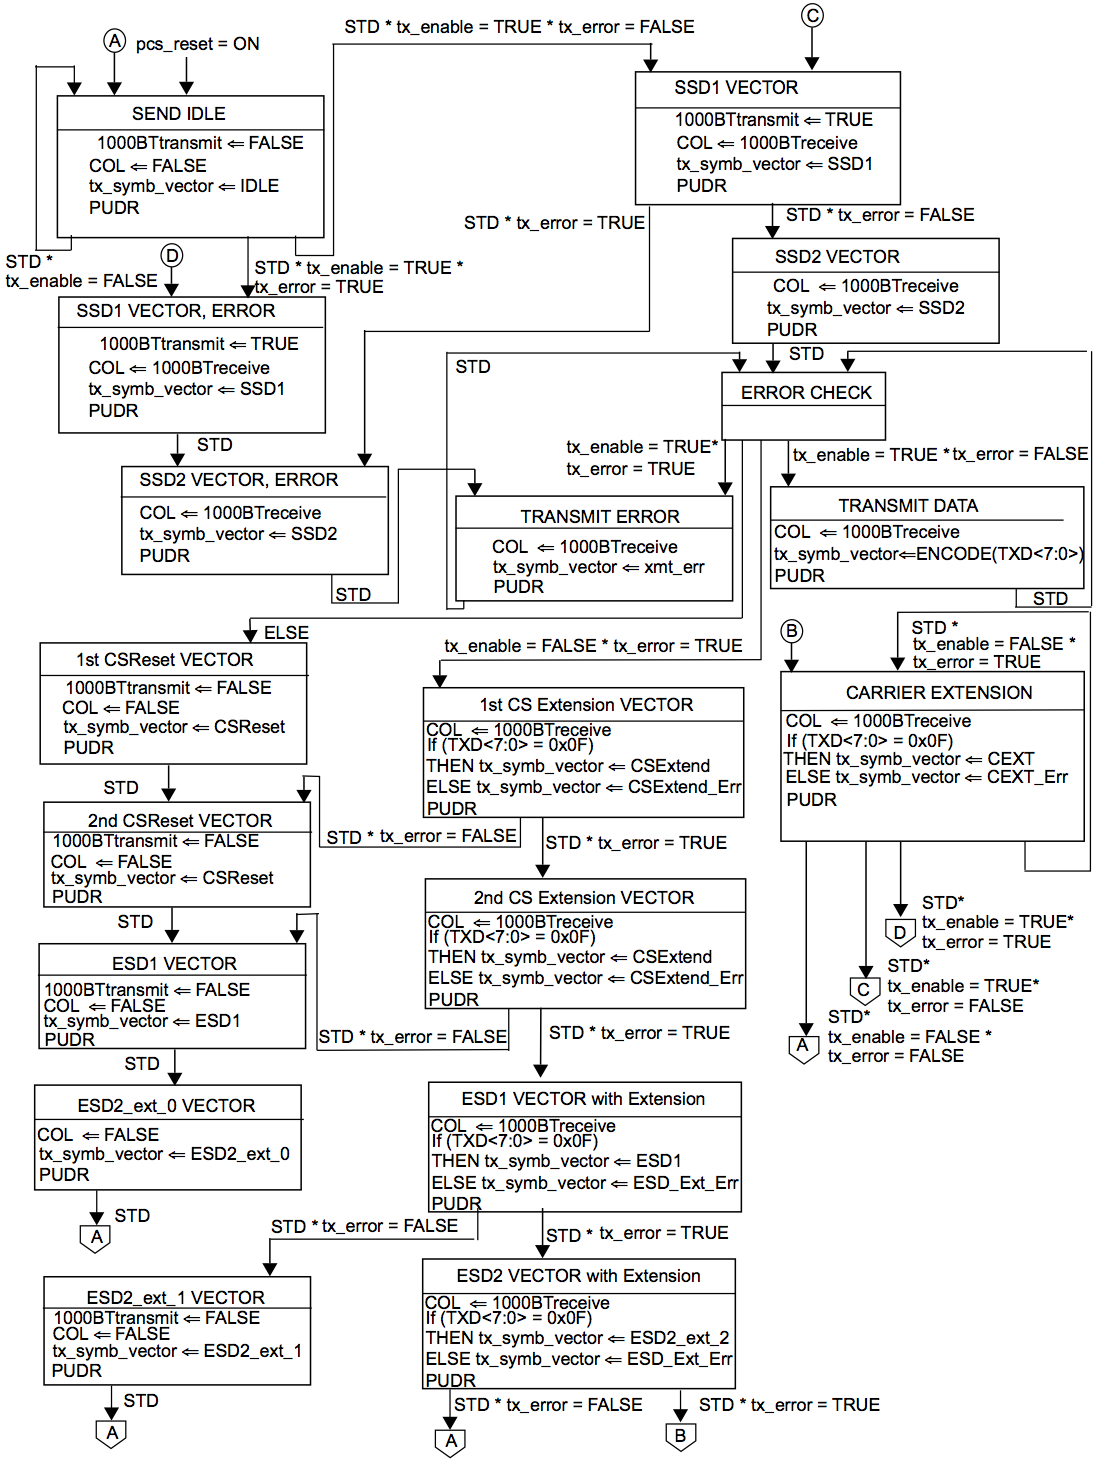
\includegraphics[width=4in]{pcs_transmit}
\caption{PCS Transmit State Diagram}
\small source:{802.3z Standard 40.3.4, Figure 40-9} \cite{802.3z}
\label{fig:pcs_transmit}
\end{figure}

Luckily though, the PCS for 1000Base-T doesn't haven't to handle collision detection since
1000Base-T is full duplex.
The PCS also uses the MII's managment interface to handle Auto-Negotiation which is required
in 1000Base-T.

\section{Data Link Layer}
The data link layer is comprised of two sublayers,
but this would be the format an operating system sees.
The layer one ethernet frame has its preamble and start of frame delimiter dropped by the MAC subsystem. Remember that the logical link layer was agnostic to the ethernet frame format.
It is only the MAC that understands which bits are which part.
\subsection{Logical Link Control}
This sublayer is higher up than the MAC and handles network control frames. It handles higher level network protocols like IP, Decnet, Appletalk, etc. We can ignore these for your ethernet subsystem.
Technically, a part flow control also resides in this sublayer,
but for LAN protocols like ethernet there is no flow control in this sublayer.
\subsection{Media Access Control (MAC)}
This sublayer interprets the bit stream into a MAC ethernet frame, checks for frame errors, and passes on the frame in its disessembled form in reception mode. When transmitting, it takes the frame, adds the preamble and start of frame delimiter and adds its own source MAC address. It is important to know that the order of transmission is by one octel at a time with the low-order bits first. Usually the MAC handles collision detection as well, and carrier sense, but since we have full-duplex you can ignore these. In short, the MAC interprets the signals from the GMII and sends the layer 2 ethernet frame to the processing system.

\chapter{Basic Approach}


\chapter{Ethernet PL IP Guide}

\chapter{PetaLinux Networking}

\chapter{Alternate Approaches}

\chapter{More on PL}

\chapter{Miscellaneous}
\section{Personal Statements}
\subsection{Dale Zhang}
For me, this class was challenging for a multitude of reasons. First off, I hadn't touched Verilog since I took 18-240 a few years ago, and I also wasn't very comfortable with HDL. In addition, in the context of our project, I had very little knowledge on ethernet and networking, so I had to learn a lot about how our project worked as I went along.

Over the course of the semester, there are definitely a few things I wish I had done differently. Since Terence and Eddie were both far more knowledgeable about Ethernet and networking, I often took a backseat to them when the group was making decisions. However, at some points in the semester, instead of asking for their help understanding some of the concepts driving our design, I would try to do it myself, without very much success. This led to me spending far more time on some tasks than I should've. This definitely limited my effectiveness as a team member.

Another mistake we made as a team was underestimating how much work actually needed to go into this project. Towards the beginning of the semester, we didn't put in much lab time outside of class periods and mandatory lab time. It first really caught up to us around mid semester with the first status meeting, where we saw how far behind we were, and how much more time we would need to commit for the rest of the semester.

Some advice I'd have for anyone planning to pursue an FPGA Ethernet project in the future is not to spend too much time trying to do research, and to start actually working on the board as soon as possible. In addition, ethernet on FPGA is not very well documented, and much of the documentation available is incorrect or incomplete.

For the class in general, it's definitely better to spend the long hours working on your project earlier in the semester, before your other classes have started to pick up. In addition, at the beginning of the semester, try and pick a project that you can be passionate about and that you would really like to see succeed. At times, I felt very unmotivated to go in an work on the project simply because I wasn't particularly excited about our final product.

To all future students reading this, good luck with the class and have fun!

\printbibliography
\appendix
\chapter{Appendix}


\end{document}
